212. \begin{figure}[ht!]
\center{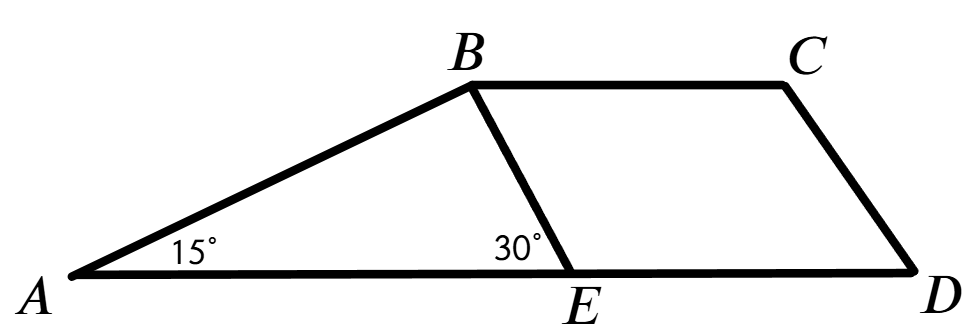
\includegraphics[scale=0.35]{g9-207.png}}
\end{figure}\\
Проведём $BE\parallel CD,$ тогда $BCDE$ является параллелограммом ($BC\parallel ED,\ BE\parallel CD),$ значит $ED=BC=\sqrt{2}$ и тогда $AE=AD-ED=2\sqrt{2}-\sqrt{2}=\sqrt{2}.$ Найдём $\angle BEA=\angle ADC=30^\circ$ как соответственные при прямых $CD$ и $BE,$ тогда $\angle ABE=180^\circ-15^\circ-30^\circ=135^\circ.$ По теореме синусов для треугольника $ABE$ имеем соотношение $\cfrac{AE}{sin(135^\circ)}=\cfrac{AB}{sin(30^\circ)},$ откуда $AB=\cfrac{\sqrt{2}}{\cfrac{\sqrt{2}}{2}}\cdot\cfrac{1}{2}=1.$\\
